\section{Node Express}
\subsection{Request Handling}

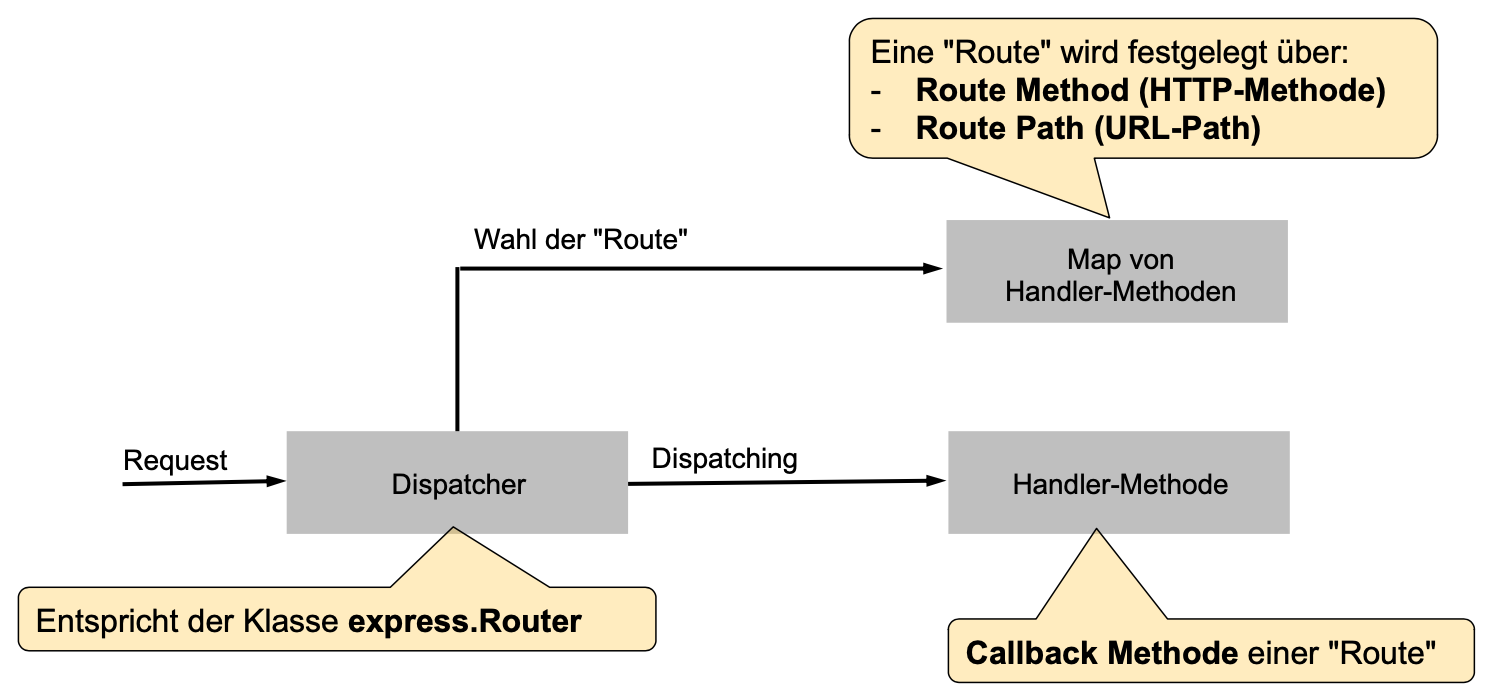
\includegraphics[width=\columnwidth]{images/noderequesthandling}
\subsection{Beispiel}
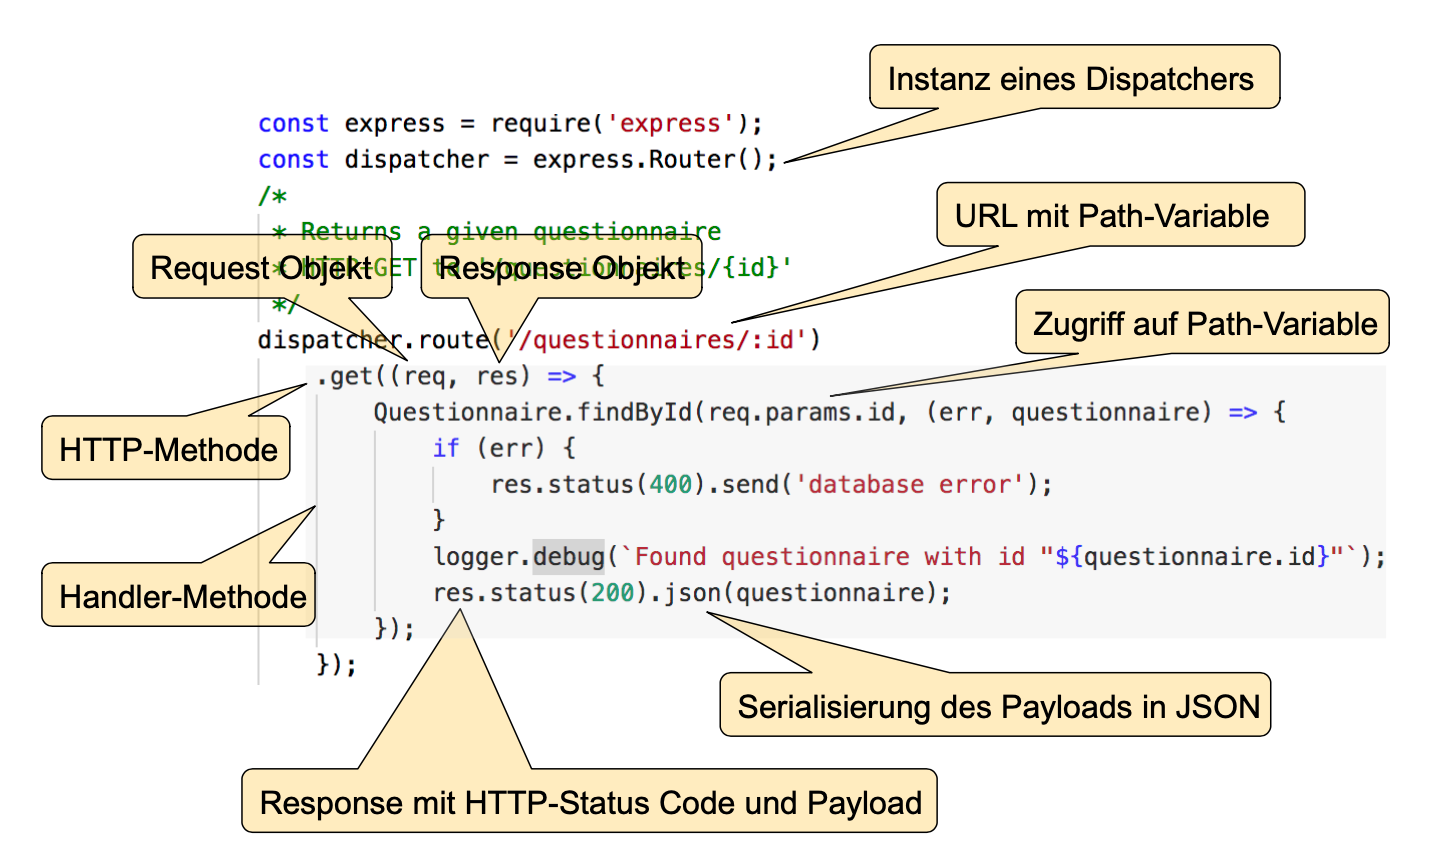
\includegraphics[width=\columnwidth]{images/requesthandlingexample}
\subsubsection{app.js}
\begin{minted}{JavaScript}
"use strict"

const log4js = require('log4js')
const dotenv = require('dotenv-extended')
const express = require('express')
const cors = require('cors')
const bodyParser = require('body-parser')
const mongoose = require('mongoose')
const routes = require('./web/dispatcher')


// Read the properties from file '.env' and '.env.defaults'
dotenv.load({ silent: true })

// Configure log4js based on the definitions in file 'log4js.json'
log4js.configure('log4js.json')
const logger = log4js.getLogger('app')

// Use native promises, needed with Mongoose since v4.1.0
mongoose.Promise = global.Promise

// Connect to the database using the connection parameters found in the property-files
const url = 'mongodb://' + process.env.MONGO_HOST + '/' + process.env.MONGO_DATABASE
logger.debug(`Database URL used '%s'`, url)
mongoose.connect(url, { useNewUrlParser: true, useUnifiedTopology: true })

// Create the Express Server App
const app = express()

// Configure body-parser. The parser handles the JSON payload.
app.use(bodyParser.json())

// Enable CORS (for all requests)
app.use(cors())

// Example how to modify the http response (see HttServletResponseWrapper in Java)
const modifyResponseBody = (req, res, next) => {
    var origSend = res.send
    res.send = body => {
        // arguments[0] (or `body`) contains the response body
        body = "modified: " + body
        origSend.apply(res, [body])
    }
    next()
}
// app.use(modifyResponseBody)

// Configure the dispatcher with all its controllers
app.use('/flashcard-express', routes)


// Read PORT from the configuration, default to 9090
const PORT = process.env.PORT || 9090

// Start the App as HTTP server
app.listen(PORT)

// Use backquotes for the es6 feature
logger.info(`Server started on port ${PORT}`)

module.exports = app
\end{minted}

\subsection{dispatcher.js}
\begin{minted}{javascript}
"use strict";

const dispatcher = require('express').Router();

const index_controller = require('./index-controller')
const questionnaire_controller = require('./questionnaire-controller')

dispatcher.route('/').get(index_controller.index)
dispatcher.route('/questionnaires').get(questionnaire_controller.findAll)
dispatcher.route('/questionnaires/:id').get(questionnaire_controller.findById)
dispatcher.route('/questionnaires').post(questionnaire_controller.create)
dispatcher.route('/questionnaires/:id').put(questionnaire_controller.update)
dispatcher.route('/questionnaires/:id').delete(questionnaire_controller.delete)

module.exports = dispatcher;
\end{minted}


\subsection{questionnaire-controller.js}
\begin{minted}{javascript}
"use strict"

const log4js = require('log4js')
const Questionnaire = require('../domain/questionnaire')

// Create a logger
const logger = log4js.getLogger('controller')

/*
 * Returns all questionnaires
 * HTTP-GET to '/questionnaires'
 */
exports.findAll = (req, res) => {
    Questionnaire.find((err, questionnaires) => {
        if (err) {
            return res.status(400).send('database error')
        }
        logger.debug(`Found ${questionnaires.length} questionnaires`)
        res.status(200).json(questionnaires)
    })
}

/*
 * Returns a given questionnaire
 * HTTP-GET to '/questionnaires/{id}'
 */
exports.findById = (req, res) => {
    Questionnaire.findById(req.params.id, (err, questionnaire) => {
        if (err) {
            return res.status(400).send('database error')
        }
        logger.debug(`Found questionnaire with id "${questionnaire.id}"`)
        res.status(200).json(questionnaire)
    })
}

/*
 * Creates a new questionnaire
 * HTTP-POST to '/questionnaires'
 */
exports.create = (req, res) => {
    // Create a new instance of the Questionnaire model
    let questionnaire = new Questionnaire()
    questionnaire.title = req.body.title
    questionnaire.description = req.body.description

    // Save the questionnaire and check for errors
    questionnaire.save((err, questionnaireCreated) => {
        if (err) {
            logger.error(`Could not create new questionnaire`)
            res.status(412).send('database error')
        } else {
            logger.debug(`Successfully created questionnaire with id "${questionnaire.id}"`)
            res.status(201).json(questionnaireCreated)
        }
    })
}

/*
 * Updates a given questionnaire
 * HTTP-PUT to to '/questionnaires/{id}'
 */
exports.update = (req, res) => {
    Questionnaire.findById(req.params.id, (err, questionnaire) => {
        if (err) {
            logger.error(`Could not update questionnaire with id "${req.params.id}"`)
            return res.status(404).send('database error')
        }
        questionnaire.title = req.body.title
        questionnaire.description = req.body.description

        // Update the questionnaire and check for errors
        questionnaire.save(err => {
            if (err) {
                return res.status(404).send('database error')
            }
            logger.debug(`Successfully updated questionnaire with id "${questionnaire.id}"`)
            res.status(200).json(questionnaire)
        })
    })
}

/*
 * Deletes a given questionnaire
 * HTTP-DELETE to '/questionnaires/{id}'
 */
exports.delete = (req, res) => {
    Questionnaire.deleteOne({ _id: req.params.id }, err => {
        if (err) {
            logger.error(`Could not delete questionnaire with id "${req.params.id}"`)
            return res.status(404).send('database error')
        }
        logger.debug(`Successfully deleted questionnaire with id "${req.params.id}"`)
        res.status(200).send()
    })
}
\end{minted}